\documentclass[11pt,a4paper]{article}
\usepackage{amsmath,amsthm,amsfonts,amssymb,amscd}
\usepackage{enumerate} 
\usepackage{physics}
\usepackage{enumerate}
\usepackage{fancyhdr}
\usepackage{hyperref}
\usepackage{graphicx}
\usepackage{xurl}
\hypersetup{colorlinks,
    linkcolor=blue,
    citecolor=blue,      
    urlcolor=blue,
}

\oddsidemargin0.1cm 
\evensidemargin0.8cm
\textheight22.7cm 
\textwidth15cm \topmargin-0.5cm

\newtheorem{theorem}{Theorem}
\newtheorem{corollary}{Corollary}
\newtheorem{lemma}{Lemma}
\newtheorem{proposition}{Proposition}

\theoremstyle{definition}
\newtheorem{remark}{Remark}
\newtheorem{definition}{Definition}
\newtheorem{observation}{Observation}
\newtheorem{note}{Note}
\newtheorem{hope}{Hope}
\newtheorem{warning}{Warning}
\newtheorem{problem}{Problem}
\newtheorem{fear}{Fear}
\newtheorem{question}{Question}

\newcommand{\Z}{\mathbb{Z}}
\newcommand{\R}{\mathbb{R}}
\newcommand{\C}{\mathbb{C}}
\newcommand{\Q}{\mathbb{Q}}
\newcommand{\A}{\mathbb{A}}

\usepackage{listings}
\usepackage{xcolor}

\definecolor{codegreen}{rgb}{0,0.6,0}
\definecolor{codegray}{rgb}{0.5,0.5,0.5}
\definecolor{codepurple}{rgb}{0.58,0,0.82}
\definecolor{backcolour}{rgb}{0.95,0.95,0.92}

\lstdefinestyle{mystyle}{
    backgroundcolor=\color{backcolour},   
    commentstyle=\color{codegreen},
    keywordstyle=\color{magenta},
    numberstyle=\tiny\color{codegray},
    stringstyle=\color{codepurple},
    basicstyle=\ttfamily\footnotesize,
    breakatwhitespace=false,         
    breaklines=true,                 
    captionpos=b,                    
    keepspaces=true,                 
    numbers=left,                    
    numbersep=5pt,                  
    showspaces=false,                
    showstringspaces=false,
    showtabs=false,                  
    tabsize=2
}

\lstset{style=mystyle}

\newcommand{\MultiSet}{\mathrm{MultiSet}}
\newcommand{\len}{\mathrm{len}}
\newcommand{\din}{\texttt{d\_in}}
\newcommand{\dout}{\texttt{d\_out}}
\newcommand{\Relation}{\texttt{Relation}}
\newcommand{\X}{\mathcal{X}}
\newcommand{\Y}{\mathcal{Y}}
\newcommand{\U}{\texttt{U}}
\newcommand{\True}{\texttt{True}}
\newcommand{\False}{\texttt{False}}
\newcommand{\clamp}{\texttt{clamp}}
\newcommand{\function}{\texttt{function}}
\newcommand{\float}{\texttt{float }}
\newcommand{\questionc}[1]{\textcolor{red}{\textbf{Question:} #1}}

\newcommand{\silvia}[1]{{ {\color{blue}{(silvia)~#1}}}}
\newcommand{\grace}[1]{{ {\color{purple}{(grace)~#1}}}}
\newcommand{\connor}[1]{{ {\color{teal}{(connor)~#1}}}}

\newcommand{\todo}{{\textcolor{red}{TODO }}}


\title{Privacy Proofs for OpenDP: Bounded Sum with Unknown $n$}
\author{S\'ilvia Casacuberta}
\date{Summer 2021}

\begin{document}

\maketitle

\tableofcontents

\section{Algorithm Implementation}
\subsection{Code in Rust}
The current OpenDP library contains the transformation \texttt{make\_bounded\_sum\_n} implementing bounded sum unknown $n$. This is defined in lines 53-68 of the file \texttt{sum.rs} in the Git repository\footnote{As of July 1, 2021.} (\url{https://github.com/opendp/opendp/blob/b936c74223b4e319698fa51837b5f8f40f3126d3/rust/opendp/src/trans/sum.rs#L53-L68}).

\begin{figure}[ht]
    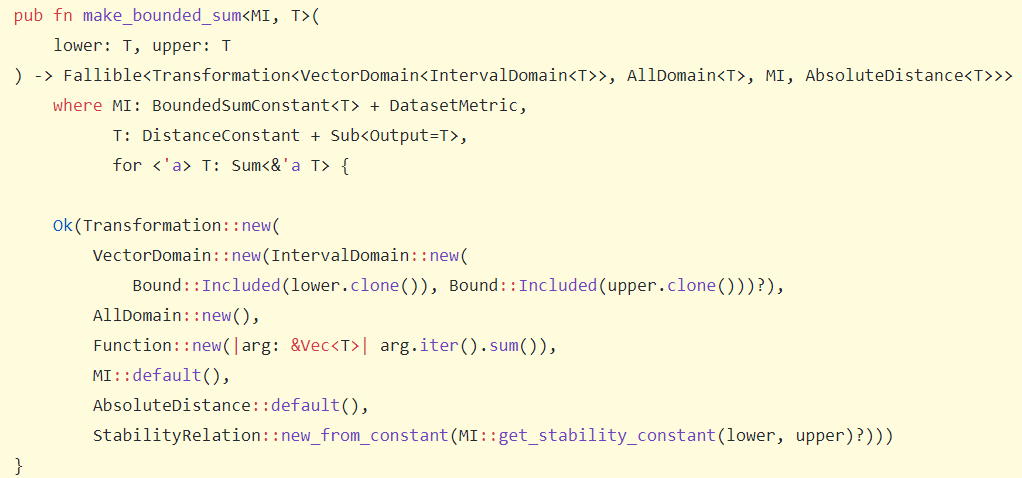
\includegraphics[width=14cm]{sum2.png}
    \centering
    \label{fig:code}
\end{figure}

\newpage

Update: after conversations with Mike about the possible overflow problems in Bounded Sum, the Rust code has been updated. The new version can be found at \url{https://github.com/opendp/opendp/blob/53e8d67b8dde4425930fb8bc397c126cd4f18370/rust/opendp/src/trans/sum.rs#L18-L33}. However, we also keep the code snippet above because this change is still a pull request and is still not part of the OpenDP library.\footnote{As of July 20.} The proof below now refers to this most updated version.

\begin{figure}[ht]
    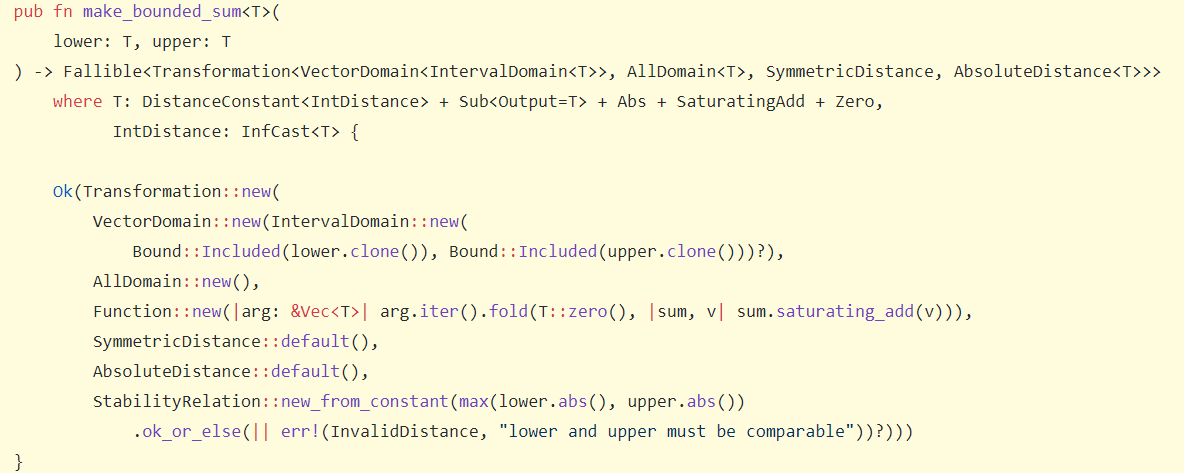
\includegraphics[width=15cm]{bounded_sum_3.png}
    \centering
    \label{fig:code}
\end{figure}

\subsection{Pseudocode in Python}
We present a simplified Python-like pseudocode of the Rust implementation below. The necessary definitions for the pseudocode can be found at \href{https://www.overleaf.com/project/60d215bf90b337ac02200a99}{``List of definitions used in the pseudocode"}.

\subsubsection*{Preconditions}
To ensure the correctness of the output, we require the following preconditions:

\begin{itemize}
    \item \textbf{User-specified types:}
    \begin{itemize}
        \item Type \texttt{T} must implement \texttt{DistanceConstant(IntDistance)}, \texttt{TotalOrd},\footnote{For now, the OpenDP library only implements \texttt{PartialOrd}, but \texttt{TotalOrd} will soon be implemented. Then, \texttt{TotalOrd} will be redundant, since the trait \texttt{TotalOrd} is part of the trait \texttt{DistanceConstant}.} \texttt{Abs}, \texttt{Sub(Output=T)}, \texttt{SaturatingAdd}, and \texttt{Zero}.
        \item \texttt{IntDistance} must have trait \texttt{InfCast(T)}. \questionc{Same question that Connor asked in \texttt{make\_count} -- this is not needed for the proof.}
\end{itemize}
\end{itemize}

\subsubsection*{Postconditions}
\begin{itemize}
    \item Either a valid \texttt{Transformation} is returned or an error is returned.
\end{itemize}

\begin{lstlisting}[language=Python, escapechar=|]
def MakeBoundedSum(L: T, U: T):
    input_domain = VectorDomain(IntervalDomain(L, U))
    output_domain = AllDomain(T)
    input_metric = SymmetricDistance()
    output_metric = AbsoluteDistance(T)
    
    def Relation(d_in: u32, d_out: T) -> bool: |\label{line:rel}|
        return d_out >= inf_cast(d_in, T) * max(abs(U), abs(L))
    
    def function(data: Vec[T]) -> T: |\label{line:fn}|
        result:T = 0
        for i in data:
            result = saturating_add(result, i) |\label{line:saturate}|
        return result
        
    return Transformation(input_domain, output_domain, function, input_metric, output_metric, stability_relation = Relation)
\end{lstlisting}

\section{Proof}
\subsection{Symmetric Distance}
\begin{theorem}
    For every setting of the input parameters \texttt{(L, U)} to \texttt{MakeBoundedSum}, the transformation returned by \texttt{MakeBoundedSum} has the following properties:
    \begin{enumerate}
        \item \textup{(Appropriate output domain).} For every vector $v$ in the input domain, $\function(v)$ is in the output domain.
        
        \item \textup{(Domain-metric compatibility).} The domain \texttt{input\_domain} matches one of the possible domains listed in the definition of \texttt{input\_metric}, and likewise \texttt{output\_domain} matches one of the possible domains listed in the definition of \texttt{output\_metric}.
        
        \item \textup{(Stability guarantee).} For every pair of elements $v, w$ in \texttt{input\_domain} and for every pair $(\din, \dout)$,  where $\din$ is of the associated type for \texttt{input\_metric} and $\dout$ is the associated type for \texttt{output\_metric}, if $v,w$ are $\din$-close under \texttt{input\_metric} and $\texttt{Relation}(\din, \dout) = \True$, then $\function(v)$, \texttt{function}$(v)$ are $\dout$-close under \texttt{output\_metric}.
    \end{enumerate}
\end{theorem}

\begin{proof}
    \textbf{(Appropriate output domain).} In the case of \texttt{MakeBoundedSum}, this corresponds to showing that for every vector $v$ in \texttt{VectorDomain(IntervalDomain(L, U))}, where \texttt{L} and \texttt{U} have type \texttt{T}, the element \texttt{function(v)} belongs to \texttt{AllDomain(T)}.
    The type signature of \texttt{function} as defined in line \ref{line:fn} automatically enforces that \texttt{function(v)} has type \texttt{T}. Since the Rust code successfully compiles, by the type signature the appropriate output domain property must hold. Otherwise, the code will raise an exception for incorrect input type. It is also necessary to check that \texttt{function(v)} is contained within the interval \texttt{[get\_min\_value(T), get\_max\_value(T)]}. This is enforced by the use of the function \texttt{saturating\_add} in line~\ref{line:saturate}, as described in \href{https://www.overleaf.com/project/60d215bf90b337ac02200a99}{``List of definitions used in the pseudocode"}.
    
    If the sum of all the vector elements in \texttt{data} is greater than \texttt{get\_max\_value(T)}, then \texttt{result} will be equal to \texttt{get\_max\_value(T)}. If the sum of all the vector elements in \texttt{data} is less than \texttt{get\_min\_value(T)}, then \texttt{result} will be equal to \texttt{get\_min\_value(T)}. Otherwise, \texttt{result} will be equal to the sum of all the vector elements in \texttt{data}, and it will be contained within the interval \texttt{[get\_min\_value(T), get\_max\_value(T)]}. Therefore, \texttt{function(v)} is guaranteed to be in \texttt{output\_domain} in all cases.
    
    \smallskip
    \textbf{(Domain-metric compatibility).} For \texttt{MakeBoundedSum}, this corresponds to showing that \texttt{VectorDomain(IntervalDomain (L, U))} is compatible with symmetric distance, and that \texttt{AllDomain(T)} is compatible with absolute distance. Both follow directly from the definition of symmetric distance and absolute distance, as stated in \href{https://www.overleaf.com/project/60d215bf90b337ac02200a99}{``List of definitions used in the pseudocode"}, along with the \textit{appropriate output domain property} shown above, which ensures that \texttt{output\_domain} is indeed \texttt{AllDomain(T)}.
    
    \smallskip
    \textbf{(Stability guarantee).} Throughout the stability guarantee proof, we can assume that $\function(v)$ and $\function(w)$ are in the correct output domain, by the appropriate output domain property shown above. 
    
    Since by assumption $\Relation(\din, \dout) = \True$, by the \texttt{MakeBoundedSum} stability relation (as defined in line~\ref{line:rel} in the pseudocode), we have that $\dout \geq \din \cdot \max{(|\texttt{U}|, |\texttt{L}|)}$. Moreover, $v, w$ are assumed to be $\din$-close. By the definition of the symmetric difference metric, this is equivalent to stating that $d_{Sym}(v, w) = |\MultiSet(v) \Delta \MultiSet(w)| \leq \din$.

    Further, applying the histogram notation,\footnote{See \textit{A Programming Framework for OpenDP}, footnote 1 in page 3. Note that there is a bijection between multisets and histograms, which is why the proof can be carried out with either notion. For further details, please consult \url{https://www.overleaf.com/project/60d214e390b337703d200982}.}  it follows that
    \[
        d_{Sym}(v, w) = \lVert h_{v} - h_{w}\rVert_1 = \sum_z |h_v(z) - h_w(z)| \leq \din.
    \]
    We want to show that
    \[
        d_{Abs}(\function(v), \function(w)) \leq d_{Sym}(v, w) \cdot \max{(|\texttt{U}|, |\texttt{L}|)}.
    \]
    This would imply that
    \[
        d_{Abs}(\function(v), \function(w)) \leq d_{Sym}(v, w) \cdot \max{(|\texttt{U}|, |\texttt{L}|)} \leq \din \cdot \max{(|\texttt{U}|, |\texttt{L}|)},
    \]
    and by the stability relation this will imply that
    \[
        d_{Abs}(\function(v), \function(w)) \leq \dout,
    \]
    as we want to see. 
\end{proof}

Let $u$ denote the vector formed by all the elements of $v$ and $w$ \textit{without multiplicities} (i.e., $u$ contains exactly once each of the elements in $\MultiSet(v) \cup \MultiSet(w)$, in any order). Let $u_i$ denote the $i$-th element of $u$, and similarly for $v$ and $w$, and let $m$ denote the length of $u$.  
Then, by definition,
\[
    d_{Sym}(v, w) = \sum_z \Big|h_v(z) - h_w(z)\Big| = \sum_i \Big|h_v(u_i) - h_w(u_i)\Big|;
\]
\[
    d_{Abs}(\function(v), \function(w)) = |\function(v) - \function(w)| \leq \Big|\sum_i v_i - \sum_i w_i\Big| = 
\]
\[
   = \Big|\sum_i u_i \cdot h_v(u_i) - \sum_i u_i \cdot h_w(u_i)\Big| = \Big|\sum_i u_i \cdot (h_v(u_i) - h_w(u_i))\Big|.
\]
Note that we have the inequality $|\function(v) - \function(w)| \leq |\sum_i v_i - \sum_i w_i|$ above (instead of an equality) due to the definition of \texttt{saturating\_add}. The equality case holds whenever $\sum_i v_i \in \texttt{[get\_min\_value(T), get\_max\_value(T)]}$ and $\sum_i w_i \in \texttt{[get\_min\_value(T),}$  $\texttt{get\_max\_value(T)]}$. In any of the possible cases where $\sum_i v_i > \texttt{get\_max\_value(T)}$ or $\sum_i v_i < \texttt{get\_min\_value(T)}$ and $\sum_i w_i > \texttt{get\_max\_value(T)}$ or $\sum_i w_i < \texttt{get\_min\_value(T)}$, the difference $|\sum_i v_i - \sum_i w_i|$ will always upper bound the value $|\function(v) - \function(w)|$, and hence it is sufficient to carry our proof by only considering the quantity $|\sum_i v_i - \sum_i w_i|$.

\silvia{Might be easier to just state this in terms of absolute clamp and refer to that transformation proof.}

By the definition of absolute distance and symmetric distance, and by applying the triangle inequality, we obtain:
\[
    d_{Abs}(\function(v), \function(w)) \leq \Big|\sum_i u_i \cdot (h_v(u_i) - h_w(u_i))\Big| \leq |u_i| \cdot \sum_i |h_v(u_i) - h_w(u_i)|.
\]
By the appropriate output domain property $u_i \in \texttt{[L, U]} \, \forall i$ it follows that $|u_i| \leq \max{(|\texttt{U}|, |\texttt{L}|)}$ for all $i$. Hence,
\[
    d_{Abs}(\function(v), \function(w)) \leq |u_i| \cdot \sum_i |h_v(u_i) - h_w(u_i)| \leq 
\]
\[
    \leq \max{(|\texttt{U}|, |\texttt{L}|)} \cdot \sum_i |h_v(u_i) - h_w(u_i)| \leq \max{(|\texttt{U}|, |\texttt{L}|)} \cdot d_{Sym}(v, w).
\]
Lastly, since by assumption $v$ and $w$ are $\din$-close, by the defined $\Relation(\din, \dout)$ (line \ref{line:fn} in the pseudocode) it follows that
\[
    d_{Abs}(\function(v), \function(w)) \leq \max{(|\texttt{U}|, |\texttt{L}|)} \cdot d_{Sym}(v, w) \leq 
\]
\[
    \leq \max{(|\texttt{U}|, |\texttt{L}|)} \cdot \din \leq \dout,
\]
as we wanted to show.

\silvia{Flag: need to account for possible rounding errors given the non-closure of float addition.}

\end{document}
